% CREATED BY DAVID FRISK, 2016
\section{Introduction}
The field of humanoid robotics is a fast growing field of research and development wherein humanoid robots are becoming more and more advanced. There are different ways for a humanoid robot to interact with the world. Walking is one of the rudimentary characteristics of human movement, achieving a bipedal walking gait allows a robot to perform more complex tasks in a world adapted for humans, but constructing a robust walking gait is not trivial. There has been a lot of research and development using Central Pattern Generators (CPGs) to construct a walking gait using Genetic Algorithms (GA) as reinforced learning method. These algorithms are known to take very long to evolve a robust walking cycle. In most projects the GA starts with a random seed, which is one of the reasons for the long time needed to evolve a good walking cylce. 


\subsection{Purpose}
The aim of this project is to investigate if using data gathered from a human walking cycle as the seed in the GA of a CPG will make the GA evolve faster and give a better walking cycle compared to using a random seed and letting it evolve from scratch. The robot used as the target platform for the movement cycle is the Bioloid robot \cite{bioloid}, shown in Figure \ref{fig:bioloid}.

\begin{figure}[htbp]
    \centering
    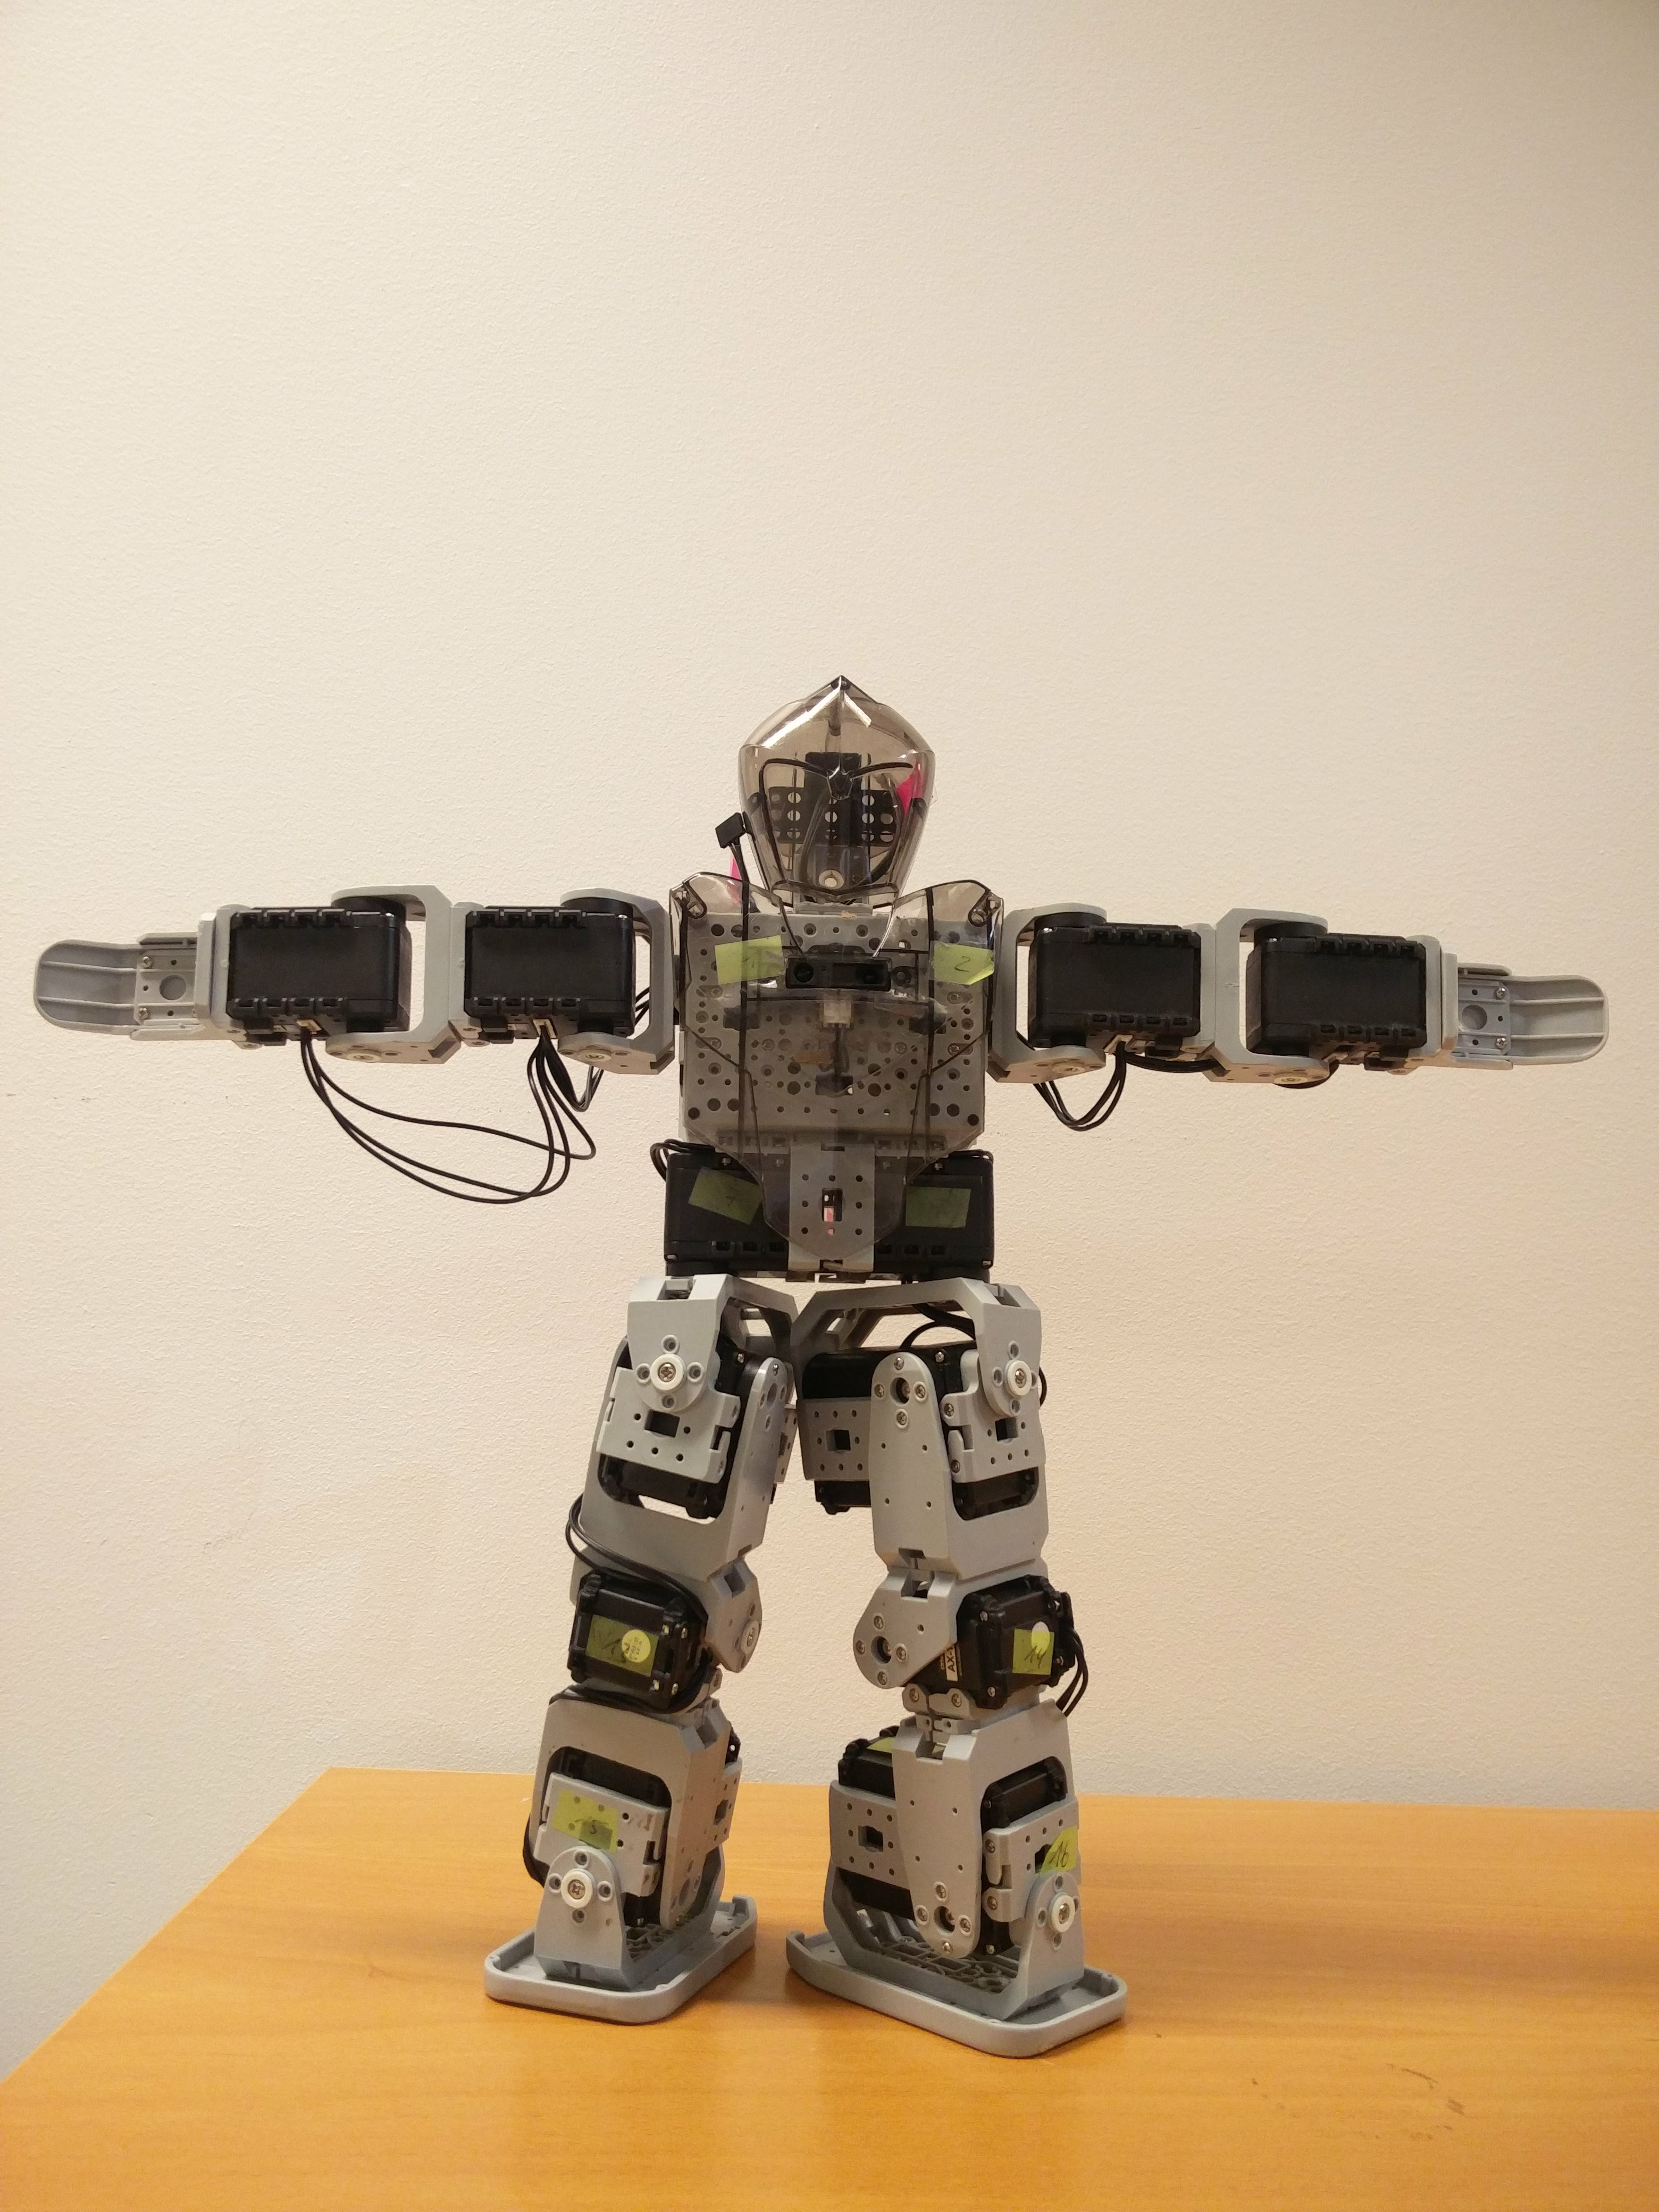
\includegraphics[width=0.35\textwidth]{include/figure/robot.jpg}
    \caption{The Bioloid robot used throughout this project.}
    \label{fig:bioloid}
\end{figure}